\documentclass[10pt,a4paper]{article}
\usepackage[margin=2cm]{geometry}
\usepackage[T1]{fontenc}
\usepackage{lmodern}
\usepackage{microtype}
\usepackage{amsmath,amssymb}
\usepackage{graphicx}
\usepackage{booktabs}
\usepackage{tabularx}
\usepackage{subcaption}
\usepackage{xcolor}
\usepackage{listings}
\usepackage{tikz}
\usetikzlibrary{positioning,calc,decorations.pathreplacing}
\usepackage[hidelinks]{hyperref}
\usepackage[capitalise,noabbrev]{cleveref}

\definecolor{nsm}{HTML}{2a78d6}
\definecolor{dsm}{HTML}{eb6834}
\definecolor{pax}{HTML}{1baf7a}
\definecolor{codebg}{HTML}{f6f5f1}
\lstset{basicstyle=\ttfamily\footnotesize, columns=fullflexible, keepspaces=true,
  backgroundcolor=\color{codebg}, frame=none, xleftmargin=4pt, xrightmargin=4pt,
  aboveskip=4pt, belowskip=4pt, language=C++, keywordstyle=\bfseries,
  commentstyle=\itshape\color{black!60}, showstringspaces=false}

\graphicspath{{figures/}}
\newcommand{\fig}[2][\linewidth]{\IfFileExists{figures/#2.pdf}{\includegraphics[width=#1]{#2}}{\fbox{\parbox{0.9#1}{\centering\small figure \texttt{#2} not generated yet (run \texttt{make figures})}}}}
\newcommand{\gen}[1]{\IfFileExists{generated/#1.tex}{\input{generated/#1.tex}}{\textit{(table \texttt{#1} not generated yet)}}}
\newcommand{\code}[1]{\texttt{#1}}
\newcommand{\ms}{\,ms}
\newcommand{\ns}{\,ns}

\title{Comparing NSM, DSM and PAX on one machine:\\ layouts, materialization, encodings and cache-aware tuning}
\author{Shaurya \quad--\quad COL868, Project 1}
\date{}

\begin{document}
\maketitle


\begin{abstract}
\noindent
We built an in-memory scan engine in C++ that stores one table as a row store (NSM), a column
store (DSM) or in PAX pages, and runs selections, projections, aggregations and full-tuple
reconstruction over it under early, late and adaptive materialization. DSM columns can also be
stored in seven encodings, with predicates and aggregates evaluated on the compressed data. On
an AMD Ryzen~5 5600H we varied projectivity, selectivity, working-set size, PAX page size,
encoding and vector size, and measured latency and hardware counters. The results reduce to
one count: the cache lines a query moves from the level of the hierarchy the data lives in,
and what the CPU does with each of them. That count explains the layout crossovers (DSM is up
to 15$\times$ faster than NSM for one attribute of 16, NSM wins full-tuple reconstruction), the
materialization crossovers (late wins below 2.4--7.4\% selectivity from DRAM, because a
gathered line costs 2.2--3.2 streamed ones), and when compression pays (when the query works on
the compressed form, e.g.\ 87$\times$ for SUM over run lengths, or when decoding costs less
than the $\approx$1 cycle of DRAM bandwidth a plain value takes, which needs AVX2). It also
tells us how to tune the engine for this machine: one hardware parameter decides one code
choice, and together they make the engine 1.46$\times$ faster over 18 query--layout pairs.
\end{abstract}

% =========================================================================================
\section{Introduction and research question}
\label{sec:intro}

The physical layout of a table decides which bytes a query has to move through the memory
hierarchy. NSM stores each tuple contiguously, so any query reads whole tuples. DSM stores
each attribute contiguously, so a query reads only the attributes it needs, but has to stitch
them back together to produce tuples. PAX~\cite{pax} keeps NSM's page as the unit of storage
but stores each attribute of the page in its own minipage, aiming for DSM's cache behaviour
with NSM's locality for reconstruction.

\paragraph{Research question.} \emph{How does the physical layout of a table, together with
the way a query turns qualifying rows into output (the materialization strategy), affect the
latency and cache behaviour of analytical queries, across projectivity, selectivity,
working-set size and PAX page size? And given the cache hierarchy of one specific machine, how
should the query code change to run faster there?}

The crossovers we study are: projectivity (how many attributes before NSM beats DSM),
selectivity (how many rows before early materialization beats late), the working-set size
(whether the answers change when the table fits in cache) and the PAX page size (how large a
page must be for PAX to scan like DSM). For the second half of the question we follow the
project's suggestion and start with \emph{early versus late materialization}, which changes
which cache lines are touched, and \emph{compression}, which changes how many values fit in
one. We then extend it to the vector size, memory placement, output writes and page size.

\paragraph{Outline.} \Cref{sec:design,sec:method} describe the engine and how we measured.
\Cref{sec:results} reports the layout experiments and \cref{sec:analysis} explains them by
counting cache lines. \Cref{sec:mat,sec:enc} apply the same count to materialization and to
encodings, \cref{sec:tuning} turns the machine's parameters into tuning rules, and
\cref{sec:tried} lists what we tried and dropped.

% =========================================================================================
\section{Design and implementation}
\label{sec:design}

\subsection{Data and layouts}

A table has $R$ rows and $N$ attributes of type \code{int64\_t}, generated once from a seeded
\code{std::mt19937\_64}. Unless stated otherwise, values are uniform in $[0, 10^6)$, so a
predicate \code{c < x} can be given any selectivity in steps of $10^{-6}$. All layouts are built
before any timing starts (\cref{fig:layouts}).

\begin{figure}[t]
\centering
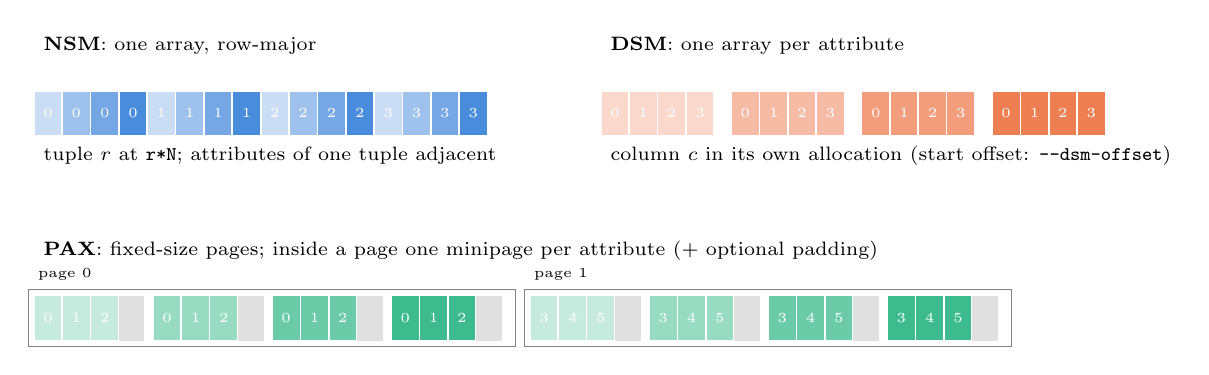
\begin{tikzpicture}[x=0.36cm,y=0.36cm,font=\scriptsize]
  % NSM
  \node[anchor=west] at (0,3.2) {\textbf{NSM}: one array, row-major};
  \foreach \r in {0,...,3} \foreach \c in {0,...,3} {
    \pgfmathtruncatemacro{\i}{\r*4+\c}
    \fill[nsm!\the\numexpr 25+\c*20\relax] (\i,0) rectangle +(1,1.6);
    \draw[white,line width=0.6pt] (\i,0) rectangle +(1,1.6);
    \node at (\i+0.5,0.8) {\tiny\textcolor{white}{\r}};
  }
  \node[anchor=west] at (0,-0.7) {tuple $r$ at \code{r*N}; attributes of one tuple adjacent};
  % DSM
  \begin{scope}[xshift=7.2cm]
  \node[anchor=west] at (0,3.2) {\textbf{DSM}: one array per attribute};
  \foreach \c in {0,...,3} \foreach \r in {0,...,3} {
    \fill[dsm!\the\numexpr 25+\c*20\relax] (\r+\c*4.6,0) rectangle +(1,1.6);
    \draw[white,line width=0.6pt] (\r+\c*4.6,0) rectangle +(1,1.6);
    \node at (\r+\c*4.6+0.5,0.8) {\tiny\textcolor{white}{\r}};
  }
  \node[anchor=west] at (0,-0.7) {column $c$ in its own allocation (start offset: \code{--dsm-offset})};
  \end{scope}
  % PAX
  \begin{scope}[yshift=-2.6cm]
  \node[anchor=west] at (0,3.2) {\textbf{PAX}: fixed-size pages; inside a page one minipage per attribute (+ optional padding)};
  \foreach \p in {0,1} {
    \draw[black!50] (\p*17.5-0.2,-0.2) rectangle +(17.2,2.0);
    \node[anchor=south west] at (\p*17.5-0.2,1.8) {\tiny page \p};
    \foreach \c in {0,...,3} {
      \foreach \r in {0,1,2} {
        \fill[pax!\the\numexpr 25+\c*20\relax] (\p*17.5+\c*4.2+\r,0) rectangle +(1,1.6);
        \draw[white,line width=0.6pt] (\p*17.5+\c*4.2+\r,0) rectangle +(1,1.6);
        \pgfmathtruncatemacro{\rr}{\p*3+\r}
        \node at (\p*17.5+\c*4.2+\r+0.5,0.8) {\tiny\textcolor{white}{\rr}};
      }
      \fill[black!12] (\p*17.5+\c*4.2+3,0) rectangle +(0.9,1.6);
    }
  }
  \end{scope}
\end{tikzpicture}
\caption{The three layouts for a table with 4 attributes (shades) and rows 0--5 (numbers).
PAX keeps page boundaries explicit: rows never span pages, every page stores its own tuple
count, and grey boxes mark the optional per-minipage padding.}
\label{fig:layouts}
\end{figure}

\begin{description}
\item[NSM] One row-major array of $R\cdot N$ values; attribute $c$ of row $r$ is at $rN + c$.
\item[DSM] $N$ arrays of $R$ values, each in its own page-aligned anonymous \code{mmap}, so that
the placement does not depend on the allocator. Column $c$ can start $c\cdot\delta$ bytes into
its allocation (\code{--dsm-offset}), which matters for cache-set conflicts
(\cref{sec:tuning:place}).
\item[PAX] Pages of a fixed size $P$ (\code{--page-size}, default 16\,KB) back to back in one
buffer. Inside a page, attribute $c$ occupies a contiguous \emph{minipage} holding that
attribute for the page's rows: with $N{=}16$, a page holds $P/128$ rows and a minipage is
$P/16$ bytes. Rows never cross pages, and no query reads across a page boundary.
\end{description}
With \code{--hugepages}, buffers of 2\,MB or more are 2\,MB-aligned and marked with
\code{madvise(MADV\_HUGEPAGE)} before they are first touched, so transparent huge pages back
them.

\subsection{Queries}

Two query classes cover what the project asks for.
\textbf{Projection}, \code{SELECT c$_{i_1}$, \dots, c$_{i_k}$ FROM t WHERE \dots}, writes the
qualifying tuples row-major into a preallocated output buffer, so every layout has to
reconstruct tuples; with all $N$ attributes it is \code{SELECT *}. \textbf{Aggregation},
\code{SELECT SUM(c$_{i_1}$)+\dots+SUM(c$_{i_k}$), COUNT(*)}, builds no tuples (AVG is SUM/COUNT).
The WHERE clause is a conjunction of predicates $\textit{lo} \le c \le \textit{hi}$, which covers
$=$, $<$, $>$ and ranges, and compiles to one unsigned comparison
$(v-\textit{lo}) \le_u (\textit{hi}-\textit{lo})$. In the sweeps, \code{--sel s} generates
\code{c0 < x} with $x$ chosen so that a fraction $s$ of the rows qualifies, and the query reads
the first $k$ attributes, so the predicate column is one of them.

\subsection{Execution: chunks, kernels and strategies}
\label{sec:design:exec}

A layout is presented to a query as a sequence of \emph{chunks} of at most $B$ rows (the vector
size, default 1024): a base pointer and a stride for NSM, or one pointer per referenced
attribute for DSM, a PAX page and a decoded vector. The kernels are templates over the chunk
type, specialised at compile time on the number of output attributes and predicates. This
matters: without it, the kernels reloaded every column pointer and predicate bound on every
row, and DSM early at $k{=}2$ ran 54 instructions per row (23.5\ms) instead of 12 (2.6\ms),
which hid every memory effect we wanted to measure. The strategies are:

\begin{description}
\item[early] Stitch, then filter. For each row, load all referenced attributes, write the
output tuple unconditionally and advance the output cursor by the predicate's 0/1 result. No
branch, and every referenced attribute of every row is read. Early SUM adds each row's
attributes and masks the row sum with the predicate result.
\begin{lstlisting}
for (i = 0; i < n; ++i) { for (j = 0; j < m; ++j) out[cnt*m + j] = col[j][i];  cnt += pass(i); }
\end{lstlisting}
\item[early-pipe] Test the predicate first and fetch the other attributes only for
qualifying rows, with one branch per row.
\item[late] Build a \emph{selection vector} of qualifying positions from the first
predicate without branches (further predicates refine it), then gather each output attribute
at those positions, one attribute at a time. Late SUM sums one column at a time over the
selection vector.
\begin{lstlisting}
for (i = 0; i < n; ++i) { sel[cnt] = i;  cnt += pass(i); }                           // select
for (j = 0; j < m; ++j)  for (t = 0; t < cnt; ++t)  out[t*m + j] = col[j][sel[t]];   // gather
\end{lstlisting}
\item[late-branch] As \emph{late}, with a branch per row in the selection.
\item[auto] Chooses \emph{early} or \emph{late} for every span of at least 1024 rows
(\cref{sec:mat:auto}).
\end{description}

\subsection{Encodings}
\label{sec:design:enc}

DSM can store each column in one of seven encodings, in blocks of 1024 values: \emph{plain};
\emph{bitpack} ($v-\min$ in the column's minimum bit width); \emph{for} (bitpack with a
per-block minimum and width, whose block minimum and maximum also form a zone map);
\emph{dict} (bit-packed codes into a sorted dictionary); \emph{dictb} (dict with codes of 1, 2 or
4 bytes); \emph{rle} ((value, run end) pairs); and \emph{delta} (bit-packed zig-zag differences).
Columns are read either one virtual call per value (\emph{value mode}, like a Volcano iterator)
or one decoded vector at a time (\emph{vector mode}). In vector mode, late strategies push
predicates into the compressed data (packed offsets compared against a translated bound, zone
maps, dictionary code ranges, one test per run), and late SUM without a predicate works on the
compressed form (\cref{sec:enc:compressed}). Early strategies decode each vector and run the
plain kernel.

\paragraph{Machine-aware knobs and correctness.} Every tuning knob is off by default, so the
defaults are an untuned baseline, and each has an \code{auto} value derived from the cache
parameters that \code{scan\_bench --machine} reads from sysfs (\cref{sec:tuning}). Before
anything is timed, every configuration runs once on every layout and strategy and is compared
with a naive row-at-a-time reference; a projection is checked with a position-weighted
checksum, so a value in the wrong row or slot is caught.

% =========================================================================================
\section{Experimental methodology}
\label{sec:method}

\paragraph{Machine.} One laptop: an AMD Ryzen~5 5600H (Zen~3, up to 4.2\,GHz) under WSL2
(Linux 6.18). Each core has a 32\,KB 8-way L1D (64 sets, so addresses 4\,KB apart share a
set) and a 512\,KB L2; the six cores share a 16\,MB L3. Lines are 64 bytes, and the widest SIMD
is AVX2 (no AVX-512). \Cref{tab:machine} gives what our microbenchmark measured on one core.
Two numbers recur. DRAM delivers about $28/4.1 \approx 7$ bytes per cycle, so a scan of 8-byte
values stays memory-bound only while it spends less than about 1.2 cycles per value. And a
store that misses first reads the line (write-allocate), so writes to DRAM reach less than half
of the read bandwidth.

\begin{table}[t]
\centering\small
\caption{The memory hierarchy measured on one core (\code{build/membench}): load-to-use latency
from a random pointer chase, bandwidth from sequential reads and writes.}
\label{tab:machine}
\gen{machine_table}
\end{table}

\paragraph{Procedure.}
\begin{itemize}
\item Only the query's \code{run()} is timed; tables, layouts, encodings and output buffers are
built and touched before. Every run is pinned to one core (\code{taskset -c 2}).
\item Each configuration gets 1 warm-up and 5 timed runs per round, over 3 rounds that
interleave all configurations, so a slow period on the host (WSL2 shares the machine with
Windows) affects all of them. We report medians.
\item The default table has $R = 4\cdot 10^6$ rows and $N = 16$ attributes: 512\,MB per
layout, 32 times the L3, so scans come from DRAM. When the table fits in a cache,
\code{--min-time-ms} repeats the scan until a sample lasts 10--20\ms.
\item DSM columns start 17 cache lines apart (\code{--dsm-offset auto}) in every experiment
except those that study placement. Page-aligned columns make row-at-a-time access to more
than 8 columns up to 3$\times$ slower (\cref{sec:tuning:place}), an artifact of allocation
that would distort every layout comparison.
\item \code{--perf} reads hardware counters (cycles, instructions, L1D accesses and misses,
dTLB misses) with \code{perf\_event\_open} around each timed run. WSL2 leaves five of Zen~3's
six counters free, so groups have at most five events. We report counters per table row.
\end{itemize}

\paragraph{Experiments.} \Cref{tab:experiments} lists them. Each is a list of
\code{scan\_bench} invocations in \code{scripts/experiments.py}, and \code{scripts/figures.py}
regenerates every figure and generated table in this report from the CSVs in \code{results/}.

\begin{table}[t]
\centering\small
\caption{Experiments. Unless noted: $R{=}4\mathrm{M}$, $N{=}16$, uniform data, PAX pages of
16\,KB, vectors of 1024 rows, DSM columns staggered by 17 lines, other knobs off.}
\label{tab:experiments}
\begin{tabularx}{\linewidth}{lX}
\toprule
Experiment & What varies \\
\midrule
projectivity & $k \in \{1,2,4,8,16\}$, no predicate; SUM and projection \\
selectivity & $s$ from 0.01\% to 100\%; projection $k\in\{2,4,16\}$ and SUM $k{=}4$; all fixed strategies; also with the table in L3 \\
width, working set & $N$ from 2 to 256 at 512\,MB; table size from 16\,KB to 512\,MB \\
PAX page & page size from 1\,KB to 4\,MB; plain, padded or odd-line minipages \\
encodings & every encoding $\times$ 5 distributions, $N{=}8$; predicates on compressed data; dictionary codes; working set; scalar and AVX2 \\
materialization & late's cost per column and per gathered line; SIMD selection from DRAM, L3, L2; auto vs early and late \\
tuning & vector size; DSM offsets and huge pages; output writes; untuned vs tuned \\
\bottomrule
\end{tabularx}
\end{table}

% =========================================================================================
\section{Results: layouts}
\label{sec:results}

% Results: the layout experiments. Why they look this way is in analysis.tex.
All latencies are medians over 15 runs, from DRAM (4M rows $\times$ 16 attributes, 512\,MB per
layout) unless the table size is the variable.

\subsection{Projectivity}
\label{sec:res:proj}

\begin{figure}[t]
\centering
\fig{projectivity}
\caption{Latency vs the number of attributes read, without a predicate. Left: SUM of $k$
attributes. Right: projection of $k$ attributes into row-major output tuples.}
\label{fig:projectivity}
\end{figure}

\Cref{fig:projectivity} varies the number $k$ of the 16 attributes a query reads.
\begin{itemize}
\item \textbf{Aggregation.} DSM's time grows in proportion to $k$, from 1.0\ms{} at $k{=}1$ to
18\ms{} at $k{=}16$, because it reads exactly $k$ arrays. NSM's hardly depends on $k$
(13--22\ms), because every row's cache lines come in anyway. At $k{=}1$ DSM is 15$\times$
faster, close to the 16$\times$ ratio of bytes moved. PAX reads only the needed minipages too,
but pays a fixed cost per minipage: 3.9\ms{} at $k{=}1$, 4$\times$ DSM (\cref{sec:res:pax}).
\item \textbf{Projection.} Every layout also writes $8k$ bytes of output per row. DSM still wins
at low projectivity (4.0\ms{} vs NSM's 19\ms{} at $k{=}1$) and up to $k{=}8$, and NSM wins at
$k{=}16$ (61\ms{} vs DSM's 72\ms{} and PAX's 79\ms). The crossover lies between $k{=}8$ and
$k{=}16$.
\item \textbf{Strategy.} Without a predicate, late is slower than early on DSM for $k \ge 2$,
by 30\% at $k{=}16$ (94 vs 72\ms), because it writes each vector's output one attribute at a
time (\cref{sec:analysis:recon}).
\end{itemize}

\subsection{Selectivity}
\label{sec:res:sel}

\begin{figure}[p]
\centering
\fig{selectivity}
\caption{Latency vs selectivity for every layout and strategy. Each row of panels is one
query; the predicate is \code{c0 < x} and $c_0$ is among the attributes read. Both axes are
logarithmic.}
\label{fig:selectivity}
\end{figure}

\begin{table}[t]
\centering
\caption{Selectivity at which late stops beating early, log-interpolated between measured
points.}
\label{tab:crossovers}
\gen{selectivity_crossovers}
\end{table}

\Cref{fig:selectivity} sweeps the selectivity of \code{c0 < x} from 0.01\% to 100\% for four
queries under the four fixed strategies, and \cref{tab:crossovers} gives where late stops
beating early.
\begin{itemize}
\item \textbf{DSM is where the strategy matters most.} At 0.01\%, late reads $c_0$ and a few
lines of the other attributes: \code{SELECT *} takes 2.3\ms{} against early's 21\ms, 9$\times$
less. Early's time is nearly flat up to about 5\%, because it always reads all $k$ attributes.
Late's grows with the selectivity and crosses early's at 2.4\% for $k{=}4$ and 7.4\% for
$k{=}16$: the more attributes late can skip, the longer it stays ahead. With $k{=}2$ there is
little to skip, and the two are within 2\% of each other from 0.5\% to 2\%. At 100\%, late is
45\% slower (99 vs 68\ms).
\item \textbf{NSM barely cares.} Every row's lines are read whatever the strategy, so the
strategies differ only in CPU work (15--23\ms{} for \code{SELECT *} at low selectivity).
\item \textbf{PAX early is slow at every selectivity} with the default 16\,KB pages:
\code{SELECT *} takes 55--63\ms{} up to 20\%, 2.6$\times$ DSM early, while PAX late follows DSM
late at a fixed offset (\cref{sec:analysis:cache}).
\item \textbf{Branches.} \emph{early-pipe} and \emph{late-branch} peak near 50\%, where the
branch is least predictable: for $k{=}2$ on DSM, late-branch takes 17.6\ms{} against late's
6.9\ms. The branch-free variants have no peak, so we use them from here on.
\item \textbf{Aggregation} has lower crossovers (DSM 1.4\%, PAX 3.3\%): early SUM writes
nothing and stays at about 3.6\ms{} on DSM, so late has less to save.
\item \textbf{Other predicates} behave like their selectivity. An equality is a range of width
one and costs what \code{c0 < x} costs at the same selectivity (7.5 vs 6.9\ms{} for DSM late
\code{SELECT *} at 1\%). A conjunction costs what its combined selectivity costs, because late
refines the selection vector with the second predicate only at the surviving positions: adding
\code{c1 = 7} to \code{c0 = 42} cuts DSM late from 7.5 to 3.0\ms.
\end{itemize}

\subsection{Table width}
\label{sec:res:width}

Keeping the table at 512\,MB while $N$ grows from 2 to 256 (so rows get wider and fewer)
changes the picture in two ways. For SUM(c0), DSM's time falls as $1/N$, while NSM's falls much
more slowly (25 to 2.1\ms), because beyond $N{=}8$ it still reads one line per row. For
\code{SELECT *} of every row, reconstruction gets more expensive for the columnar layouts as
rows widen (DSM 63\ms{} at $N{=}4$, 106\ms{} at $N{=}256$; PAX 68 to 131\ms), while NSM's
row-major copy stays at 66--69\ms. Beyond about 16 streams, neither the 8-way L1 nor the
prefetcher keeps up with stitching $N$ columns. At 1\% selectivity NSM becomes the fastest from
$N{=}128$ (4.8 vs 5.2\ms{} for DSM): each qualifying row is then a short contiguous range,
while DSM fetches one line per qualifying row from each of $N$ columns.

\subsection{Working-set size}
\label{sec:res:ws}

\begin{figure}[t]
\centering
\fig{workingset}
\caption{Time per row vs table size ($N{=}16$), from 16\,KB (in L1) to 512\,MB. Dotted lines
mark the cache capacities. Small tables are scanned repeatedly until a sample lasts 20\ms.}
\label{fig:workingset}
\end{figure}

\Cref{fig:workingset} varies the table size from 16\,KB to 512\,MB.
\begin{itemize}
\item \textbf{SUM(c0)} costs DSM 0.08--0.10\,ns per row from L2 and L3 and 0.26\,ns from
DRAM, and NSM 0.5--0.6\,ns in cache and 3.8\,ns from DRAM. The NSM/DSM ratio grows from about
5$\times$ in L2 to 15$\times$ in DRAM: in cache the difference is CPU work (a strided load per
row against vectorized contiguous loads), in DRAM it is bytes.
\item \textbf{SUM of all 16 attributes.} From DRAM every layout moves the same 128 bytes per
row (4.3--5.5\,ns). In cache NSM is twice as slow as DSM (2.5 vs 1.1--1.4\,ns), because summing
across a row vectorizes worse than summing down a column.
\item \textbf{\code{SELECT *}.} DSM is the fastest while the table fits in L2 or a quarter of
L3 (2.2--3.1\,ns per row against NSM's 3.1--3.5), and NSM once the table fills L3 (13.0 vs
13.6\,ns at 16\,MB, 16.1 vs 18.1\,ns from DRAM). The reconstruction crossover depends on
where the data lives, not only on the layout.
\item Going from a 4\,MB table (in L3) to DRAM costs 2.3--5.8$\times$ for every query and
layout, more than any layout difference for wide queries.
\end{itemize}

\subsection{PAX page size}
\label{sec:res:pax}

\begin{figure}[t]
\centering
\fig{pax_pagesize}
\caption{PAX latency vs page size: plain packing, 64 bytes of padding after each minipage,
and an odd-line minipage stride (\code{--pax-pad auto}). Horizontal lines: DSM with the same
query and strategy. The predicate on $c_0$ passes 1\% or all rows.}
\label{fig:pax}
\end{figure}

\Cref{fig:pax} varies the PAX page size from 1\,KB to 4\,MB. A minipage is $P/16$ bytes: 64
bytes at 1\,KB, 1\,KB at the default 16\,KB, 256\,KB at 4\,MB.
\begin{itemize}
\item \textbf{One attribute} (SUM(c0)) gets faster as pages grow: 20.1\ms{} at 1\,KB, 4.9 at
16\,KB, 2.8 at 64\,KB and 1.2 at 4\,MB, which equals DSM. At 16\,KB the excess over DSM is
3.7\ms{} over 31{,}250 pages, about 120\,ns per page, roughly one DRAM latency.
\item \textbf{\code{SELECT *} at 1\%.} Late falls from 12.9\ms{} at 16\,KB to 6.5\ms{} at
256\,KB, reaching DSM late (7.1\ms). Early with plain packing stays at 38--66\ms{} at every
size, 1.7--2.9$\times$ DSM early (22.7\ms), and gets \emph{worse} from 64\,KB (65.6\ms) as
pages grow; with an odd-line minipage stride it drops to 23--28\ms.
\item \textbf{\code{SELECT *} of every row.} Late is fastest with tiny pages (71--72\ms{} at
1--2\,KB, 86--101\ms{} from 16\,KB): a page of 8 tuples keeps a vector's output tile in L1.
\item \textbf{64 bytes of padding} per minipage changes nothing from 16\,KB up and wastes
space below.
\end{itemize}
So the PAX page size trades the prefetcher, which wants long minipages, against
reconstruction locality, which wants small pages. The 8--16\,KB pages of disk-based PAX are on
the wrong side of it for scans in memory. \Cref{sec:analysis:cache} explains both effects and
\cref{sec:tuning} fixes them.


% =========================================================================================
\section{Analysis: counting cache lines}
\label{sec:analysis}

% Analysis: why the layout results look the way they do.

\subsection{The cache-line count}
\label{sec:analysis:lines}

Almost every result in \cref{sec:results} follows from one quantity: the number of cache lines
a query moves per table row, from the level of the hierarchy the table lives in.
\Cref{tab:linemodel} lists it for 8-byte values in 64-byte lines ($v = 8$ values per line), $N$
attributes, $k$ read and selectivity $s$. The central term is
\[
  f(s) = 1 - (1-s)^{v},
\]
the fraction of a column's lines that hold at least one selected value: a line is skipped
only if all $v$ of its values fail. A late strategy cannot avoid those lines, even though it
wants one value from each.

\begin{table}[t]
\centering\small
\caption{Cache lines moved per table row ($v{=}8$). The predicate is on one of the $k$
attributes. Output lines are written; without streaming stores each one is also read first.}
\label{tab:linemodel}
\begin{tabular}{lll}
\toprule
 & input lines per row & output lines per row (projection) \\
\midrule
NSM, any strategy & $\lceil N/8 \rceil$ (whole rows; 2 for $N{=}16$) & $s\,k/8$ \\
DSM / PAX, early & $k/8$ & $s\,k/8$ \\
DSM / PAX, late & $1/8 + (k-1)/8 \cdot f(s)$ & $s\,k/8$ \\
\bottomrule
\end{tabular}
\end{table}

\begin{figure}[t]
\centering
\fig{selectivity_lines}
\caption{Measured L1D misses per row (markers) vs the input-line model of
\cref{tab:linemodel} (grey) for \code{SELECT * WHERE c0 < x}, from DRAM.}
\label{fig:sellines}
\end{figure}

\paragraph{The model against the counters.} \Cref{fig:sellines} compares measured L1D misses
per row with the model for \code{SELECT *} on DSM and PAX. Early misses 2.2 times per row
against a predicted 2. Late follows $1/8 + 15/8\,f(s)$ up to about 2\% (0.128 measured vs
0.127 predicted at 0.01\%, 0.32 vs 0.27 at 1\%); above that, the misses of its output tile
take over (\cref{sec:analysis:recon}).

\paragraph{Lines predict time.} From DRAM a streamed line costs about $64\,\text{B} /
28\,\text{GB/s} \approx 2.3$\,ns, and a written line about $64/12 \approx 5.3$\,ns because of the
read for ownership.
\begin{itemize}
\item NSM \code{SELECT *} at $k{=}N{=}16$: the model gives $4\mathrm{M} \cdot (2 \cdot 2.3 + 2
\cdot 5.3)\,\text{ns} = 61$\ms; we measured 61.2\ms.
\item SUM: NSM moves 2 lines per row at every $k$ (13--22\ms), DSM $k/8$ (about $1.0 \cdot
k$\ms). Hence the 15$\times$ at $k{=}1$, close to the 16$\times$ ratio of lines.
\item The projectivity crossover is where DSM's $k/8$ input lines plus its reconstruction
overhead exceed NSM's 2: between $k{=}8$ and 16.
\item In cache, lines are cheap (\cref{tab:machine}), so the same counts predict much smaller
differences: the NSM/DSM ratio for SUM(c0) shrinks from 15$\times$ in DRAM to 5$\times$ in L2.
What is left is CPU work.
\end{itemize}
By the input lines alone, late should beat early at every $s < 1$, since
$1/8 + (k-1)/8\,f(s) < k/8$. It does not, and \cref{sec:mat} measures the two costs the count
leaves out.

\subsection{When the CPU, not memory, is the limit}
\label{sec:analysis:cpu}

At 4.1\,GHz DRAM delivers about 7 bytes per cycle and L2 about 31. A loop that spends more
cycles per byte than that is CPU-bound, and its layout matters less than its instruction
count. Three cases showed up in the counters: generic tuple-at-a-time code (54 instructions
per row before the kernels were specialised, \cref{sec:design:exec}); early on 16 attributes,
which copies all 16 values of every row (54 instructions and 22 cycles per row on DSM, so its
21\ms{} in \cref{fig:selectivity} is partly CPU time, not only the 18\ms{} it takes to stream
512\,MB); and everything in cache, where summing 16 attributes takes 1.1\,ns per row on DSM
and 2.5\,ns on NSM, both far from the L2's bandwidth.

\subsection{Cache behaviour beyond line counts}
\label{sec:analysis:cache}

Four effects change the cost of a line without changing how many are moved. Each is tied to
one parameter of this machine, and \cref{sec:tuning} turns each into a fix.
\begin{description}
\item[Short streams and the prefetcher.] The hardware prefetcher detects a stream after a few
misses and does not follow it across a 4\,KB page. A DSM column is one long stream; a PAX
minipage of a 16\,KB page is a stream of 16 lines, followed by a jump of 15\,KB to the next
page's minipage. That is the 120\,ns per page of SUM(c0) on PAX (\cref{sec:res:pax}): each
minipage starts with a trip to DRAM. Early reads all 16 minipages of a page row by row, 16
short streams at once, and pays about 1\,\textmu s more per page than DSM (\code{SELECT *} at
1\%: 53.8 vs 22.7\ms). Late reads one minipage at a time and pays less. The smallest pages
avoid the problem differently: a 1\,KB page has 16 one-line minipages, so reading it row by row
is one sequential stream through the table, and its cost becomes per-page CPU work instead.
\item[Set conflicts (L1: 64 sets $\times$ 8 ways, stride 4\,KB).] Addresses 4\,KB apart share an
L1 set. Page-aligned DSM columns, and PAX minipages from 64\,KB pages up (stride $P/16$, a
multiple of 4\,KB), put value $r$ of all 16 attributes in one 8-way set. Reading them in
lockstep, as early does, evicts lines that are still needed: 8.6 L1D misses per row instead of
about 3, and early \code{SELECT *} at 1\% nearly three times slower (\cref{sec:tuning:place}).
\item[TLB reach.] With 4\,KB pages, the 2048-entry L2 dTLB covers 8\,MB, a quarter of one 32\,MB column.
A scan of 16 columns misses it 0.063 times per row, and late, which works through one column at
a time, cannot overlap the page walks with other loads (\cref{sec:tuning:pages}).
\item[Write-allocate.] A store that misses reads the line before overwriting it, so output
lines cost about twice the DRAM traffic of input lines (12 vs 28\,GB/s). Streaming stores avoid
the read, but only for whole lines written in order (\cref{sec:tuning:output}).
\end{description}

\subsection{Tuple reconstruction}
\label{sec:analysis:recon}

To build an output tuple of $k$ attributes, DSM and PAX gather from $k$ places, while NSM copies
one contiguous range. This costs in three ways.
\begin{enumerate}
\item \textbf{Streams.} Early reads $k$ input streams and writes one output stream at once.
Beyond about 16 streams the L1's 8 ways and the prefetcher's stream table run out, which is
why DSM's \code{SELECT *} grows with the width while NSM's does not (\cref{sec:res:width}).
\item \textbf{The output tile.} Late writes a vector's output one attribute at a time, so each
output line is touched $v$ times and the tile of $B \cdot k \cdot 8$ bytes must stay cached
between touches. With $B{=}1024$ and $k{=}16$ it is 128\,KB: too big for L1 (19 misses per
row), small enough for L2. With $B{=}65536$ it is 8\,MB, spills L2, and the time nearly
doubles.
\item \textbf{Instructions.} A gather is a load of the position, a load of the value and a
strided store, about 7 instructions per value against about 3 for early. This is why late is
slower than early at 100\% even when the bytes moved are the same (99 vs 68\ms{} on DSM).
\end{enumerate}
NSM pays none of these: its reconstruction is a copy. It still loses at low projectivity and
selectivity, because it reads every row's lines. Hence the classic split: DSM (late) wins when
few attributes or few rows are wanted, NSM wins \code{SELECT *} over many rows, and PAX tracks
DSM only once its pages are large and its minipages do not alias.


% =========================================================================================
\section{Early or late materialization}
\label{sec:mat}

% Early vs late: what late pays for, the threshold, cache, and choosing per chunk.

Late materialization reads the predicate column in full, and of every other column only the
lines that hold a selected row. Early streams every referenced column in full. This section
measures why late's smaller line count does not always win, turns that into a threshold, and
shows how the answer changes when the data is in cache.

\subsection{What late pays for}
\label{sec:mat:cost}

\begin{table}[t]
\centering\small
\caption{Lines late reads from one gathered column, per 8{,}000 rows (1{,}000 lines of 8
values). Lines $= 1000 \cdot f(s)$.}
\label{tab:linecount}
\begin{tabular}{rrrr}
\toprule
Selected & Values wanted & Lines read & Values brought in \\
\midrule
1\% & 80 & 77 & 616 \\
5\% & 400 & 337 & 2{,}696 \\
10\% & 800 & 570 & 4{,}560 \\
\bottomrule
\end{tabular}
\end{table}

\paragraph{Late reads lines, not values.} \Cref{tab:linecount} shows how fast $f(s)$ grows. At
1\% late touches 8\% of a column's lines, at 5\% a third, at 10\% more than half, while it wants
only one value from each. Two further costs, which the line count of \cref{tab:linemodel}
leaves out, decide where late stops winning. We separated them by timing late and early on DSM
for $k = 1$ to 16 at 0.01--10\% (\code{results/late\_breakdown/}).
\begin{itemize}
\item \textbf{A fixed first pass.} Building the selection vector with scalar code costs about 2
cycles per row, against about 1.2 for streaming 8 bytes from DRAM. Late with $k{=}1$ at
0.01\% takes 2.05\ms{} for 4M rows. With the AVX2 selection vector (\cref{sec:mat:cache}) it
takes 1.21\ms, the time of one bare column read, so the scalar pass is CPU-bound and costs
about 0.7 column scans more than reading $c_0$.
\item \textbf{A gathered line costs more than a streamed one}, 2.2--3.2 times per touched line.
A gathered column takes 0.34\ms{} at 1\% (8\% of its lines), 0.66\ms{} at 2.4\% (18\%),
1.17\ms{} at 5\% (34\%) and 1.97\ms{} at 10\% (57\%), against 1.27--1.63\ms{} for a whole
column in early. Gathered lines are sparse and irregular, so the prefetcher cannot run ahead of
them, and each is a separate DRAM access limited by latency and the number of misses in flight.
At 5\%, gathering a third of a column (1.28\ms{} with $k{=}2$) already takes longer than
reading all of it (1.21\ms).
\end{itemize}
The first pass is paid once per query, and every column late skips pays some of it back. That
is why the crossover grows with $k$: 1.6\% for $k{=}2$, 2.4\% for $k{=}4$, 7.4\% for $k{=}16$
(\cref{tab:crossovers}).

\subsection{A threshold from the line size}
\label{sec:mat:threshold}

In units of one sequential column scan per row, early costs $1 + g$ and late
$1 + \sigma + g\,f(s)/\varphi$, where $g$ is the number of attributes late gathers, $1/\varphi$
the cost of a gathered line relative to a streamed one, and $\sigma$ late's fixed cost. Late
wins while
\[
  f(s) < \varphi\,(1-\sigma/g)
  \quad\Longleftrightarrow\quad
  s < 1-\bigl(1-\varphi(1-\sigma/g)\bigr)^{1/v}.
\]
The machine enters through $v = \text{line size}/\text{value width}$. Fitted to the DSM
crossovers from DRAM, $\varphi = 0.55$ and $\sigma = 2$, and the rule predicts 2.5\% for $g=3$
and 7.8\% for $g=15$, against 2.4\% and 7.4\% measured. The two constants are a joint fit, not
the costs measured one at a time (0.7 scans and 2.2--3.2$\times$): the model charges early a
constant cost per column and assumes a constant $\varphi$, which the measurements do not, and
with the measured values it would predict 4.4\% and 5.5\%. The rule also shows two things.
Late can never win when $g \le \sigma$, i.e.\ when it skips at most two attributes, and for
$g=1$ late is indeed at most 18\% faster. And packing more values into a line lowers the
threshold: a 10-bit column holds 51 values per line, so $f(1\%)$ is already 0.40
(\cref{sec:enc:compressed}).

\subsection{In cache, instructions per row decide}
\label{sec:mat:cache}

\begin{table}[t]
\centering
\caption{Selectivity at which late stops beating early with the table in L3 (4\,MB, compare
\cref{tab:crossovers}).}
\label{tab:crossovers_cache}
\gen{selectivity_cache_crossovers}
\end{table}

\begin{table}[t]
\centering\small
\caption{Where late stops beating early on DSM ($k{=}4$), with the scalar and the AVX2
selection vector.}
\label{tab:simdcross}
\gen{simd_crossovers}
\end{table}

With the table in L3 (\cref{tab:crossovers_cache}), the crossovers move apart in opposite
directions. Projections favour late much longer: 20\% instead of 2.4\% for $k{=}4$ on DSM, 33\%
instead of 7.4\% for $k{=}16$, because a gathered line now costs an L3 hit instead of a DRAM
access, while early still pays the CPU time of copying every row. SUM goes the other way: late
never wins on DSM or PAX.

The reason is that cache shrinks early's cost far more than late's. For SUM of 4 DSM columns,
early's cost is bytes: 4.4 cycles per row from DRAM, 1.2 in L3 (0.30\,ns), where the reads are
about three times faster and early's masked sum (\code{total += row\_sum \& mask}: no branch,
no store, the same work for every row) is vectorized by the compiler. Late's first pass is
instructions: about 2.1 cycles per row from DRAM and 1.9 in L3 (0.46\,ns). In L3, late spends
more on building the selection vector alone than early spends on the whole query, so it loses
even at 0.01\%, where it skips almost every line.

\paragraph{A hand-written SIMD selection vector.} The compiler cannot vectorize the selection
loop, although the build allows AVX2 (\code{-march=native}). Its output is a packed list:
where row $i$ goes depends on how many earlier rows passed (a stream compaction), so the lanes
of a register cannot be processed independently. Our AVX2 kernel compares 8 values with two
4-lane 64-bit compares (\code{vpcmpgtq}, signed only, so the sign bit is flipped to make the
range test unsigned), turns the result into an 8-bit mask (\code{movemask}), loads the
positions of the set bits from a 256-entry table (8\,KB, stays in L1), adds the vector offset,
stores all 8 and advances the output index by \code{popcount}(mask). AVX2 has no compress
instruction; AVX-512's \code{vpcompressd} would replace the table, but Zen~3 has no AVX-512.
\begin{itemize}
\item In cache the first pass drops from about 2 to 0.9 cycles per row (0.46 to 0.20\,ns in
L3, 0.51 to 0.24 in L2), now below early's 1.2, and late SUM wins up to 3.4\% in L3 and 5.8\%
in L2 (\cref{tab:simdcross}).
\item From DRAM, late is memory-bound and gains about a third only at the lowest
selectivities (the first pass falls from 2.05 to 1.21\ms); the crossovers move from 1.2--2\% to
about 3\%.
\item Early does not use a selection vector and is unchanged.
\end{itemize}

\subsection{Choosing per chunk}
\label{sec:mat:auto}

\begin{table}[t]
\centering\small
\caption{Auto against the better of early and late at each of 10 selectivities, with the table
in L3: geometric mean / worst point over NSM, DSM and PAX (1.00 is always right).}
\label{tab:autocache}
\begin{tabular}{lccc}
\toprule
Query & DRAM constants & in-cache constants & measured (\cref{sec:tried}) \\
\midrule
SUM, $k{=}4$ & 1.19 / 1.68 & 1.20 / 1.55 & 1.09 / 1.16 \\
\code{SELECT} $k{=}4$ & 1.06 / 1.35 & 1.05 / 1.20 & 1.06 / 1.12 \\
\code{SELECT *} & 1.13 / 2.58 & \textbf{1.02 / 1.30} & 1.06 / 1.10 \\
\bottomrule
\end{tabular}
\end{table}

\emph{auto} applies the threshold to every span of at least 1024 rows, using the selectivity of
the previous span. Spans are at least 1024 rows because a 128-row PAX page at 1\% holds 0 to 4
qualifying rows, too few to estimate a selectivity from.
\begin{itemize}
\item \textbf{Where the constants were fitted it is enough.} From DRAM on uniform data, auto is
within 1\% of the better fixed strategy on NSM and DSM at every selectivity (geometric mean);
always running late would cost 21\% on DSM, always early 42\%.
\item \textbf{On sorted data it beats both fixed strategies}, by 10\% on DSM on average and by
up to 24\% (\code{SELECT *} at 10\%). The qualifying rows form one contiguous stretch, so
late is right outside it and early inside, and choosing per span gets both.
\item \textbf{The constants depend on where the data lives.} In L3, the DRAM constants pick
early for \code{SELECT *} at 10--20\%, 2.3--2.6$\times$ too slow. Since the engine knows the
table's size, \code{--auto-cache} switches to a second pair, fitted on the in-cache runs
($\varphi = 1$, $\sigma = 2$: a gathered line costs about a streamed one), whenever the table
fits in L3. That brings \code{SELECT *} to 1.02 on average and 1.30 at worst
(\cref{tab:autocache}).
\item \textbf{The remaining misses need more constants.} In cache, early SUM vectorizes and
early \code{SELECT} does not, so one pair cannot fit both, and SUM stays up to 1.55$\times$ off.
On PAX from DRAM, whose early strategy is slower than DSM's, \code{SELECT *} is up to
2.4$\times$ off. A threshold per query class and layout would fix both, at the price of more
fitted constants.
\end{itemize}


% =========================================================================================
\section{Encodings}
\label{sec:enc}

% Encodings: decoding first loses, computing on compressed data wins, and the decode budget.

\begin{table}[t]
\centering\small
\caption{Compression ratio (uncompressed bytes / encoded bytes) per data set.}
\label{tab:encratio}
\gen{encodings_ratio}
\end{table}

Each data set has one encoding it is meant for (\cref{tab:encratio}): uniform values in
$[0,100)$ for bitpack, for and dict (7 bits, 9.1$\times$; dictb's 1-byte codes 8.0$\times$);
sorted values for delta (15.6$\times$) and for (5.3$\times$); runs of mean length 64 for rle
(32$\times$); Zipf values from 10{,}000 distinct ones for dict (4.5$\times$, dictb 4.0$\times$);
and \emph{wide} 64-bit values, where nothing compresses. The table has $N{=}8$ attributes and
4M rows, from DRAM.

\subsection{Decoding first never pays off}
\label{sec:enc:decode}

\begin{table*}[t]
\centering\small
\caption{Speedup over plain DSM, best strategy, scalar / AVX2 kernels. Above 1 the encoding is
faster than the uncompressed column.}
\label{tab:encspeed}
\resizebox{\textwidth}{!}{\gen{encodings_speedup}}
\end{table*}

The early strategy decodes every vector and then runs the plain kernel. With scalar code it is
slower than plain DSM for every encoding, whatever the compression: SUM of all 8 attributes
runs at 0.80$\times$ for bitpack (9.1$\times$ smaller), 0.69$\times$ for rle (32$\times$
smaller), 0.30$\times$ for delta (15.6$\times$) and 0.30$\times$ for dict. The speed does not
follow the compression ratio, because the scan is no longer limited by bytes but by the
instructions that decode them. Value mode, one virtual call per value, is 5--11$\times$ slower
than plain for every encoding, plain included.

\subsection{Computing on the compressed form}
\label{sec:enc:compressed}

\begin{table}[t]
\centering\small
\caption{Decoding first vs working on the compressed form (ms, AVX2 kernels). SUM rows: all 8
attributes, on the encoding's own data set. Zone maps and dict: SUM(c0) with a predicate at
0.1--1\%.}
\label{tab:encdecode}
\begin{tabular}{llrrr}
\toprule
Encoding & Operation on the compressed form & decode first & compressed & plain \\
\midrule
rle & $\sum$ value $\times$ run length & 11.5 & \textbf{0.10} & 8.4 \\
delta & $m f + \sum_k d_k (m-k)$ per block & 24.5 & \textbf{6.4} & 8.0 \\
bitpack & $m \cdot \min + \sum$ offsets & 7.7 & \textbf{4.9} & 7.9 \\
for & zone maps skip blocks (sorted) & 4.0 & \textbf{0.09--0.36} & 1.3--1.4 \\
dict & compare 14-bit codes (unpacked first) & 2.6 & 1.63 & \textbf{1.28} \\
\bottomrule
\end{tabular}
\end{table}

Without a predicate, late SUM on an encoded column calls one aggregate that works on the
compressed data, so the work scales with the compressed size, not the number of values
(\cref{tab:encdecode}).
\begin{itemize}
\item \textbf{rle} adds value $\times$ run length once per run: 0.10\ms, 87$\times$ faster than
plain DSM. The first version took 1.9\ms, because a binary search for the first run of every
1024-row vector took 60\% of the time (each vector covers only about 16 runs). Remembering the
run the previous vector ended in, one call per column when there is no predicate, and a loop
over whole runs that gcc vectorizes brought it to 0.10\ms. The 7.6\,MB of runs then stay in L3
between repetitions, which is part of the 87$\times$.
\item \textbf{delta} sums each block from its deltas, $m f + \sum_k d_k(m-k)$, without the
prefix sum that rebuilds the values. The prefix sum is a dependency chain through every value
(3--4 cycles per value); the formula has none, and the AVX2 kernel computes it with two
running sums per lane: 6.0--6.4\ms, 1.25--1.31$\times$ faster than plain.
\item \textbf{Predicates on packed data.} bitpack and for compare packed offsets against a
translated bound and extract the other attributes only at selected positions. With 10-bit
values a line holds 51 of them, so late gathers 6.4 times fewer lines, and late SUM on bitpack
beats every uncompressed plan up to 5\% (2.4\ms{} at 1\% against 2.7 for late and 3.6--3.9 for
early on plain DSM). The same packing lowers the crossover within one encoding, 5--10\% for
SUM on bitpack and for against 17--21\% for the uncompressed column, because $f(s)$ is already
0.40 at 1\% (\cref{sec:mat:threshold}).
\item \textbf{Zone maps.} On sorted data, for skips every block whose minimum and maximum
exclude the predicate and accepts every block they include: 0.09--0.36\ms{} at 0.1--1\%,
against 1.3--1.4\ms{} for late on plain DSM and 4.0\ms{} for decoding first.
\end{itemize}

\subsection{Dictionary codes that fit a SIMD lane}
\label{sec:enc:dictb}

\begin{table*}[t]
\centering\small
\caption{\code{SUM WHERE c0 < x} on Zipf data in ms: plain DSM, dict (14-bit packed codes) and
dictb (2-byte codes), best of early and late, AVX2. The selectivities are those the Zipf data
allows.}
\label{tab:encdict}
\gen{enc_dict}
\end{table*}

dict is the exception in \cref{tab:encdecode}: working on its codes still loses (1.63 vs
1.28\ms{} at 1\%), because each code is stored in exactly $\lceil\log_2 |D|\rceil = 14$ bits and
has to be unpacked into a 32-bit lane before the cheap comparison. dictb rounds the code width
up to 1, 2 or 4 bytes, a lane width AVX2 compares directly. A predicate is then one
subtraction, one unsigned minimum and one comparison per 16 two-byte codes read straight from
memory, and \code{movemask} gives one bit per code. It costs 12\% of the compression
(4.5$\times$ to 4.0$\times$) and turns the dictionary predicate from a loss into a win
(\cref{tab:encdict}): 0.57\ms{} at 1\%, 2.2$\times$ faster than plain and 2.9$\times$ faster
than dict, and 5.4$\times$ faster than plain at 0.05\%. The gain shrinks as more is gathered
(0.9$\times$ at 41\%, where every selected row still needs a lookup), and scalar code gets
nothing from the byte layout (1.9\ms{} at every selectivity).

\subsection{When decoding must happen: a budget per value}
\label{sec:enc:budget}

\begin{table}[t]
\centering\small
\caption{SUM of 8 attributes on uniform data, cycles per value, by where the uncompressed table
would live. Packed: bitpack and for with the AVX2 fused unpack-and-add.}
\label{tab:budget}
\begin{tabular}{lrrr}
\toprule
Table in & Plain & Packed (AVX2) & Packed vs plain \\
\midrule
L2 / L3 & 0.26--0.30 & 0.61--0.68 & 0.40--0.49$\times$ \\
16\,MB (spilling L3) & 0.46 & 0.61--0.68 & 0.72--0.76$\times$ \\
DRAM & 0.90--0.98 & 0.61--0.68 & \textbf{1.42--1.60$\times$} \\
\bottomrule
\end{tabular}
\end{table}

Where the values must be decoded, decoding and loading overlap, so the time per value is
\[
  t = \max(\text{compute},\ \text{load}),\qquad
  \text{packed wins when}\ \max(\text{decode}+\text{add},\ \text{load}_\text{packed})
  < \max(\text{add},\ \text{load}_\text{plain}).
\]
From DRAM the packed load is small (9$\times$ less data), so packed wins when decoding plus
adding costs less than loading a plain value: about 1 cycle per 8-byte value at 28\,GB/s. In
cache the plain load is cheap and the budget shrinks to 0.26--0.30 cycles. The measurements
follow it (\cref{tab:budget}).
\begin{itemize}
\item \textbf{Scalar unpacking} of 7-bit values costs 1.2--1.3 cycles per value, just over the
DRAM budget: bitpack moves 9.1$\times$ fewer bytes and is still 0.8$\times$ as fast as plain.
\item \textbf{AVX2 unpacking with a fused sum} costs 0.61--0.68 cycles per value at every size.
In the format we use, 8 consecutive $w$-bit values occupy exactly $w$ bytes; for $w \le 25$,
one byte shuffle places each value's bytes in its own 32-bit lane and a per-lane variable
shift (\code{vpsrlvd}, AVX2 only) and a mask extract it, and the offsets are added without
being stored. From DRAM that is within the budget, and bitpack and for become
1.56--1.60$\times$ faster than plain on uniform data; in cache it is twice the plain cost.
\item \textbf{Dictionary decoding} adds a dependent lookup per value (2--4 cycles), over the
budget even with SIMD unpacking. A dictionary pays off for predicates, not for decoding.
\end{itemize}
So on this machine compression is a way to make a DRAM-bound scan CPU-bound, and it pays off
only from DRAM and only with SIMD decoding: the deciding size is the L3 capacity, measured on
the uncompressed table.


% =========================================================================================
\section{Tuning for this machine}
\label{sec:tuning}

% Tuning: one machine parameter -> one code choice, and the result of all of them together.

The analysis tied each effect to one parameter of this machine. This section turns each
parameter into a rule that \code{scan\_bench} applies when the corresponding knob is set, and
measures what it buys (\cref{tab:tuning}). The rules are computed at start-up from sysfs, so
nothing in the code is specific to this laptop; the constants of the materialization threshold
(\cref{sec:mat}) were fitted on it.

\begin{table*}[t]
\centering\small
\caption{Machine parameters and the choices derived from them.}
\label{tab:tuning}
\begin{tabularx}{\textwidth}{>{\raggedright}p{3.3cm}>{\raggedright}p{2.5cm}Xp{3.7cm}}
\toprule
Parameter (this machine) & Decides & Rule & Measured effect \\
\midrule
Line size (64\,B), value width; where the table lives & early or late, per span &
late while $f(s) < \varphi(1-\sigma/g)$, with constants for DRAM and for tables that fit in L3
(\cref{sec:mat:auto}) & within 1\% of the better fixed strategy on DSM from DRAM; \code{SELECT *}
in L3 worst case 2.6$\times$ $\to$ 1.3$\times$ \\
Cache sizes vs work per value & vector size & fit the vector's buffers in L2 ($\frac14$) for
our scans; smaller for random access inside a vector, larger for a high fixed cost per vector &
decoding SUM 1.2$\times$ faster than an L1-sized vector (\cref{sec:tuning:batch}) \\
L1 set stride (4\,KB), 64 sets, 8 ways & DSM column starts, PAX minipage stride & column $c$
starts $17c$ lines into its page; minipages hold an odd number of lines & early \code{SELECT *}
at 1\%: 2.7$\times$ on DSM, 2.3--2.7$\times$ on PAX (\cref{sec:tuning:place}) \\
Write-allocate (12\,GB/s, 40 with NT stores) & how output is written & build each vector's
tuples in a cache-resident stage, copy it out with streaming stores & projections of every row
1.2--1.9$\times$ faster (\cref{sec:tuning:output}) \\
Prefetcher (stops at 4\,KB pages); dTLB reach (8\,MB) & PAX page size; OS page size & 256\,KB
PAX pages; 2\,MB pages for buffers of 2\,MB or more & PAX SUM(c0) 4.5 $\to$ 1.2\ms; late SUM
20\% faster (\cref{sec:tuning:pages}) \\
AVX2 (no compress, no AVX-512); DRAM at 7\,B/cycle & selection and decoding kernels; code width
& hand-written SIMD selection vector and fused unpack-and-add; dictionary codes of 1, 2 or 4
bytes & late SUM wins in cache; bit-packed SUM 1.6$\times$ faster than plain; dictionary
predicate 2.2--5.4$\times$ (\cref{sec:mat:cache,sec:enc}) \\
\bottomrule
\end{tabularx}
\end{table*}

\subsection{Vector size: match it to the work, not to one cache level}
\label{sec:tuning:batch}

\begin{table}[t]
\centering\small
\caption{ns per value for three synthetic workloads and our decoding scan, with the vector's
buffers sized to fit L1, L2 or L3 (\code{build/batchbench}, \code{results/batch\_demo/}). Best
per row in bold.}
\label{tab:batchwork}
\begin{tabular}{lrrr}
\toprule
Workload & fits L1 & fits L2 & fits L3 \\
\midrule
random reads inside the vector & \textbf{1.34} & 1.69 & 2.55 \\
random reads + 2\,\textmu s per vector & 2.40 & \textbf{1.90} & 2.60 \\
light work + 20\,\textmu s per vector & 12.05 & 2.26 & \textbf{1.69} \\
our scan (decode 8 bit-packed columns + SUM) & 0.37 & \textbf{0.31} & 0.32 \\
\bottomrule
\end{tabular}
\end{table}

The engine processes one vector of $B$ rows at a time, and the vector's buffers (selection
vector, decoded values, output tile) live in L1, L2 or L3 depending on $B$. Two costs pull in
opposite directions: the work per value, which is cheaper when the buffers sit in a faster
level, and the fixed cost per vector (a decode call per column, loop setup, a prefetcher
restart, or in other systems a call into another runtime or a hand-off to another thread),
which a larger vector amortises. \Cref{tab:batchwork} shows that either can win.
\begin{itemize}
\item \textbf{Random reads inside the vector} (like probing a per-vector table) want L1: L1
answers in about 4 cycles, L2 in 12.
\item \textbf{The same with 2\,\textmu s per vector} wants L2: an L1-sized vector pays the fixed
cost too often.
\item \textbf{Light work with 20\,\textmu s per vector} wants L3 or more: the fixed cost
dominates until the vector is megabytes large.
\item \textbf{Our scans} read their buffers sequentially, and an L2 hit streams at 130\,GB/s,
nearly L1's 122, so L1-sized vectors cut L1D misses but not time. Late \code{SELECT *} at
100\% with 128-row vectors keeps its output tile in L1 and cuts misses from 19 to 5 per row,
at the same latency. But small vectors slow decoding (one call per column per vector):
bit-packed SUM takes 11.9\ms{} with the 128 rows an L1-sized rule gives, and 9.9\ms{} with
1024. Beyond the L2 the buffers spill and both slow down again.
\end{itemize}
So \code{--batch auto} sizes the vector so that every byte it touches per row fits in a quarter
of L2, $B = \max\{2^i : 2^i \cdot b_\text{row} \le L2/4\}$, leaving room for lines in flight and
prefetched lines. On this machine that is 256 rows for \code{SELECT *} of 16 attributes, 1024
for 4, and 1024 for decoding 8 bit-packed columns. A workload with random accesses inside the
vector, or a large fixed cost per vector, would need the rule moved to L1 or to L3.

\subsection{Placing columns and minipages in the cache sets}
\label{sec:tuning:place}

\begin{table}[t]
\centering\small
\caption{Early \code{SELECT *} at 1\% on PAX, plain minipages vs an odd number of lines per
minipage (\code{--pax-pad auto}); L1D misses per row in brackets.}
\label{tab:aliasing}
\begin{tabular}{lrr}
\toprule
Page size (minipage stride) & plain & odd-line minipages \\
\midrule
32\,KB (2\,KB: 8 per set, fits) & 37.8\ms & not needed \\
64\,KB (4\,KB) & 65.6\ms{} (8.6) & 27.8\ms{} (3.3) \\
256\,KB & 63.0\ms & 24.2\ms \\
4\,MB & 62.7\ms & 23.3\ms \\
\bottomrule
\end{tabular}
\end{table}

Streams read in lockstep must not share an L1 set (\cref{sec:analysis:cache}). Two rules
follow from the 64 sets and the 4\,KB set stride.
\begin{itemize}
\item \textbf{DSM} (\code{--dsm-offset auto}): column $c$ starts $17c$ lines into its
page-aligned allocation. 17 is coprime to the 64 L1 sets and the 1024 L2 sets, so up to 64
columns fall into distinct L1 sets. Early \code{SELECT *} at 1\% drops from 62.6 to 22.9\ms.
\item \textbf{PAX} (\code{--pax-pad auto}): from 64\,KB pages up, the 16 minipages start $P/16$
apart, a multiple of 4\,KB, so value $r$ of all of them maps to one set. Shortening each
minipage to an odd number of lines (64 $\to$ 63 at 64\,KB) puts them in 16 different sets, at a
cost of one line per minipage (1.6\%). Early \code{SELECT *} at 1\% becomes 2.3--2.7$\times$
faster, within 7\% of DSM from 256\,KB pages (\cref{tab:aliasing}). Padding by 64 bytes does
not help: with the page size fixed, the stride stays $P/16$.
\end{itemize}
The effect is largest where reading dominates. Early is the only strategy that reads the 16
streams at once (late reads one at a time and is unaffected), and at 1\% almost nothing is
written. At 100\%, where writing the output dominates, the misses still halve but the time
improves only 1.1$\times$ (90.8 to 81.9\ms{} at 64\,KB), and SUM of 16 attributes, which is
bound by DRAM bandwidth, also gains only 1.1$\times$ (20.0 to 18.4\ms).

We found the effect by accident. DSM columns first came from \code{malloc}, and depending on
the allocator's state they were either carved back to back out of the heap (which happened to
spread them over 16 sets) or given one page-aligned \code{mmap} each. The same \code{SELECT *}
took 21\ms{} in one experiment and 64\ms{} in another. The engine now gives large buffers
their own \code{mmap} and staggers DSM columns explicitly.

\subsection{Writing the output}
\label{sec:tuning:output}

\begin{table}[t]
\centering\small
\caption{Three ways to write a projection's output.}
\label{tab:stage}
\begin{tabular}{lcc}
\toprule
Approach & absorbs scattered writes? & avoids the read before write? \\
\midrule
normal stores & yes (the cache does) & no, paid per line \\
streaming stores directly & no (partial lines) & yes \\
stage (normal stores) + streaming copy & yes & yes \\
\bottomrule
\end{tabular}
\end{table}

\begin{table}[t]
\centering\small
\caption{Projections of every row (ms) with direct writes, a stage copied with \code{memcpy}, and
a stage copied with streaming (NT) stores.}
\label{tab:outputknobs}
\resizebox{\linewidth}{!}{\gen{output_knobs}}
\end{table}

A projection of every row writes as many bytes as it reads, and from DRAM those writes cost
more: a normal store that misses reads the line first, so writes reach 12\,GB/s while reads
reach 28. Streaming (non-temporal) stores skip that read: they fill a 64-byte write-combining
buffer in the core and send the whole line to memory, at 40\,GB/s. But only whole lines written
in order benefit, and our writes are scattered: early writes each row's slot and overwrites it
when the row fails, late writes a vector's output one attribute at a time. So
\code{--nt-stores} lets each vector write its tuples with normal stores into a small stage that
stays in cache, and copies the stage out with 32-byte streaming stores (\cref{tab:stage}).
\begin{itemize}
\item At 100\% this makes every configuration 1.2--1.9$\times$ faster
(\cref{tab:outputknobs}): DSM early 71.2 to 37.9\ms, NSM early 67.1 to 41.5\ms, and PAX late,
whose column-at-a-time writes were the most scattered, 86.5 to 45.3\ms. The line model predicts
it: 512\,MB read at 28\,GB/s and written at 40\,GB/s take 31\ms{} if nothing overlaps, against
61\ms{} with write-allocate.
\item The stage alone (\code{memcpy}) is up to 36\% slower than writing directly: it adds a
copy and still pays for write-allocate. The gain comes from the streaming stores.
\item At 1\% there is almost nothing to write, and the three modes are within noise.
\end{itemize}
Streaming stores bypass the cache, so they suit a result written once and read later. A result
consumed right away by the next operator should stay in cache.

\subsection{Pages: the prefetcher and the TLB}
\label{sec:tuning:pages}

\paragraph{PAX page size.} Every PAX minipage is a new stream that the prefetcher has to find
(\cref{sec:analysis:cache}), about 120\,ns per page at 16\,KB. Larger pages make the minipages
longer: SUM(c0) takes 4.9\ms{} at 16\,KB, 2.8 at 64\,KB and 1.2 at 4\,MB, the same as DSM. The
tuned configuration uses 256\,KB pages with odd-line minipages, where late \code{SELECT *}
reaches DSM late and early comes within 7\% of DSM early.

\paragraph{Huge pages.} The 2048-entry L2 dTLB covers 8\,MB with 4\,KB pages, so a 32\,MB column
needs 8192 translations, and 16 with 2\,MB pages. With \code{--hugepages}, buffers of 2\,MB or
more are allocated 2\,MB-aligned and marked \code{MADV\_HUGEPAGE} before they are first touched
(WSL2's kernel backs only such marked regions with huge pages). For SUM of 16 DSM columns, dTLB
misses fall from 0.031 to 0.008 per row for both strategies, but only late gets faster: 23.3 to
18.7\ms{} (20\%), against 19.3 to 18.8\ms{} (3\%) for early. Early's 16 interleaved columns keep
other loads going while one of them waits for a page walk; late works through one column at a
time, so its single stream stalls on every walk. Staggering helps early, huge pages help late.

\subsection{Everything together}
\label{sec:tuning:all}

\begin{figure}[t]
\centering
\fig{tuned}
\caption{Six queries with the untuned defaults (light) and with every machine-derived knob
(dark), best strategy of each, 4M rows from DRAM.}
\label{fig:tuned}
\end{figure}

\begin{table*}[t]
\centering\small
\caption{Untuned against tuned, in ms. Untuned: 1024-row vectors, page-aligned DSM columns,
4\,KB pages, direct output writes, scalar kernels, 16\,KB PAX pages, and the best of the four
fixed strategies. Tuned: \code{--batch auto --dsm-offset auto --hugepages --nt-stores --simd},
256\,KB PAX pages with \code{--pax-pad auto}, and auto (in this run measuring both strategies,
\cref{sec:tried}). Speedups are over the untuned best.}
\label{tab:tuned}
\gen{tuned}
\end{table*}

\Cref{fig:tuned,tab:tuned} put the knobs together on six queries and three layouts, from DRAM.
The untuned engine is given the best of the four fixed strategies per cell, which a real engine
cannot know in advance; the tuned one has to pick its strategy with auto.
\begin{itemize}
\item \textbf{Over the 18 cells the tuned engine is 1.46$\times$ faster} (geometric mean;
1.50$\times$ with the best tuned strategy): 1.11$\times$ on NSM, 1.41$\times$ on DSM and
1.96$\times$ on PAX, up to 3.8$\times$ for PAX SUM(c0) (4.5 to 1.2\ms).
\item \textbf{Projections of many rows gain on every layout}: \code{SELECT *} of every row
1.7$\times$ on NSM, 2.3$\times$ on DSM and 2.5$\times$ on PAX, mostly from the streaming stores.
After tuning NSM no longer wins it: 36.9\ms, against 34.6 on DSM and 31.7 on PAX.
\item \textbf{PAX gains the most}, because two of its defaults are wrong for memory: 16\,KB pages
are too short for the prefetcher, and larger pages alias in L1 without the odd-line stride.
\item \textbf{Queries that already move few lines gain little}: DSM SUM(c0) is one sequential
stream (1.03$\times$).
\item \textbf{Exceptions.} NSM \code{SELECT *} at 10\% (0.95$\times$): its best untuned
strategy, early-pipe, is not in the tuned set. PAX at 10\% is unchanged. One cell, NSM
\code{SELECT c0..c3} at 1\% with auto (0.76$\times$), hit a slow period on the host; repeated
three times, auto takes 15.2--16.1\ms{} against late's 14.5--15.4, and the 1.46$\times$ includes
the bad measurement.
\end{itemize}


% =========================================================================================
\section{Tried and dropped}
\label{sec:tried}

% Ideas we implemented and measured, and why they were not kept (or kept only in part).

\begin{description}
\item[Measuring both strategies instead of a threshold.] With \code{--auto-measure}, auto times
every span of at least 1024 rows with \code{rdtsc}, keeps a moving average of each strategy's
cycles per row for each power-of-two range of selectivity, and runs the cheaper one, re-running
the other now and then (once every $32\times$ its cost ratio spans) to refresh its estimate. Two
details were needed. About one span in 250 is interrupted and takes 3--30 times its cost, so
samples are clipped at twice the running estimate; without that, one spike made auto pick the
wrong strategy for hundreds of spans. And deciding per 128-row PAX page cost about a cycle per
row. It works: from DRAM it stays within 5\% of the better fixed strategy (geometric mean),
and in L3 its worst point is 1.16$\times$ (\cref{tab:autocache}). We did not keep it as the
rule, because it costs 2--5\% where the threshold is already right (the timing and the
exploration), 5--15\% in cache, where a span of early SUM takes only about 1{,}200 cycles, and
a threshold that knows where the data lives gets most of its benefit for free. It remains as an
option, and the tuned run of \cref{tab:tuned} used it.
\item[One gather pass for all columns.] Late makes one pass over the selection vector per
output attribute. A variant that makes one pass and writes all $k$ attributes of each selected
row (more independent misses per row, output written in order) took 0.97--1.11 times as long
below 5\%: the per-attribute loop already keeps many misses in flight, since each address comes
from the cached selection vector. Above 7\% it was 10--30\% faster, but there late already loses,
and it moved the $k{=}16$ crossover only from about 7\% to 8--9\%. The expensive part is the
touched line, not how the loop is organised.
\item[Vectors sized to L1.] Our first rule kept a vector's data in half of the L1D. It cut L1D
misses but not time, and made decoding 1.2$\times$ slower (\cref{sec:tuning:batch}).
\item[Padding PAX minipages by 64 bytes.] Meant to break the L1 aliasing of large pages, it
changed nothing: with the page size fixed, padding lowers the tuples per page and the stride
stays $P/16$. An odd number of lines per minipage is what works (\cref{sec:tuning:place}).
\item[A stage copied with \code{memcpy}.] Up to 36\% slower than writing directly. Only the
streaming copy makes the stage worthwhile (\cref{sec:tuning:output}).
\item[SUM over dictionary codes by counting.] Counting each code's occurrences and multiplying
by the dictionary once was 10--25\% slower than one lookup per row, with 32-bit counters and
with 16-bit L1-resident ones: a counter update is a load, an add and a store, and rows with the
same code wait for each other through memory. dictb's SUM without a predicate stays at 9.3\ms,
against 8.2\ms{} for plain.
\item[Skipping empty code groups in dictb.] A branch that skips 32-code groups without a match
is predictable only while matches are rare. At 1\% selectivity 27\% of the groups hold one, and
the branch doubled the scan time. dictb skips empty groups only when the previous vector's
selectivity was below 0.2\%, and is branch-free otherwise.
\end{description}


% =========================================================================================
\section{Conclusions}
\label{sec:conclusions}

On one core of this laptop, every result reduces to the cache lines a query moves from the
level of the hierarchy the data lives in, and to what the CPU does with each line.

\paragraph{Layouts.} DSM wins whenever a query reads few attributes or produces few rows: up to
15$\times$ over NSM for one attribute of 16, and up to 9$\times$ over its own early strategy for
\code{SELECT *} at 0.01\%. NSM wins the reconstruction of many attributes over many rows,
because its reconstruction is a copy, and it is the least sensitive to strategy, width and
placement. PAX matches DSM only with large pages: with the 8--16\,KB pages of disk-based PAX its
minipages are too short for the prefetcher, and from 64\,KB on they alias in L1 unless their
stride is an odd number of lines. Where the data lives moves the strategy crossovers by an order
of magnitude, while the layout ranking stays the same.

\paragraph{Materialization.} Late reads, of every attribute it gathers, the fraction
$1-(1-s)^v$ of lines holding a selected value, and each gathered line costs 2.2--3.2 streamed
ones from DRAM. It wins below 2.4\% (4 attributes) to 7.4\% (16) from DRAM, and up to 20--33\%
for projections in L3, where gathered lines are cheap; in cache the CPU work per row decides,
and late SUM wins only with a hand-written SIMD selection vector. A threshold from the line size
and two fitted constants, chosen by where the table lives, picks between them per span and beats
both fixed strategies on clustered data.

\paragraph{Encodings.} Fewer bytes alone do not make a scan faster: decoding first was slower
than plain for every encoding, even rle with 32$\times$ fewer bytes. Compression wins when the
query works on the compressed form (SUM over runs 87$\times$, SUM from deltas 1.3$\times$, zone
maps up to 15$\times$ over late on plain, byte-aligned dictionary codes 2.2--5.4$\times$).
Otherwise it wins only if decoding costs less than the time memory takes per plain value, about
1 cycle from DRAM and 0.3 in cache: here that requires AVX2, and only pays from DRAM.

\paragraph{Tuning.} One hardware parameter decides one code choice: the line size and where the
data lives decide the materialization threshold, the cache sizes and the work per value decide
the vector size, the L1 set stride decides where columns and minipages start, write-allocate
decides how output is written, the prefetcher and the TLB decide the PAX and OS page sizes, and
the SIMD width and DRAM bandwidth decide the kernels and the code width. Together they make the
engine 1.46$\times$ faster over 18 query--layout pairs, up to 3.8$\times$, without changing the
queries.

\paragraph{Limitations.} All results come from one core of one laptop under WSL2, with 8-byte
integer attributes. The rules use parameters that sysfs reports, but the constants of the
threshold were fitted here, and the size of each effect depends on this machine; on another
machine they should be measured again with \code{make experiments}.


\begin{thebibliography}{9}
\bibitem{pax} A.~Ailamaki, D.~J.~DeWitt, M.~D.~Hill, M.~Skounakis.
\newblock Weaving relations for cache performance.
\newblock In \emph{VLDB}, 2001.
\bibitem{abadi} D.~J.~Abadi, D.~S.~Myers, D.~J.~DeWitt, S.~R.~Madden.
\newblock Materialization strategies in a column-oriented DBMS.
\newblock In \emph{ICDE}, 2007.
\bibitem{x100} P.~Boncz, M.~Zukowski, N.~Nes.
\newblock MonetDB/X100: Hyper-pipelining query execution.
\newblock In \emph{CIDR}, 2005.
\bibitem{lemire} D.~Lemire, L.~Boytsov.
\newblock Decoding billions of integers per second through vectorization.
\newblock \emph{Software: Practice and Experience}, 45(1), 2015.
\end{thebibliography}

\end{document}
